

\documentclass{article}

\usepackage{graphicx}			% Use this package to include images
\usepackage{amsmath}			% A library of many standard math expressions
\usepackage[margin=0.75in]{geometry}% Sets 1in margins. 
\usepackage{fancyhdr}			% Creates headers and footers
\usepackage{enumerate}          %These two package give custom labels to a list
\usepackage[shortlabels]{enumitem}
\usepackage{tikz}
\usepackage{float} % Add this in your preamble for using [H]

\usepackage{booktabs}
\usepackage{caption}
\usepackage[normalem]{ulem}
\useunder{\uline}{\ul}{}

\usepackage{ragged2e} % Package for justification
\justifying

\graphicspath{{img/}}


\def\mytitle{Homework 1}
\def\righthead{EEF205E}


\usepackage[T1]{fontenc}
\usepackage{lmodern}

%%%%%%%%%%%%%%%%%%%%%%%%%%%%%%%%%%%%%%%%%%%%%%%%%%%%%%%%
\pagestyle{fancy}
\fancyhead[l]{Rüzgar Erik}
\fancyhead[c]{\mytitle}
\fancyhead[r]{\righthead}
\fancyfoot[c]{\thepage}
\renewcommand{\headrulewidth}{0.2pt}
\setlength{\headheight}{15pt}
%%%%%%%%%%%%%%%%%%%%%%%%%%%%%%%%%%%%%%%%%%%%%%%%%%%%%%%%
\usepackage{parskip}
\setlength{\parindent}{0pt} % Disable paragraph indentation
%%%%%%%%%%%%%%%%%%%%%%%%%%%%%%%%%%%%%%%%%%%%%%%%%%%%%%%%


\usepackage{listings}
\usepackage{xcolor}

\lstdefinestyle{verilogstyle}{
    language=Verilog,
    backgroundcolor=\color{white},
    basicstyle=\ttfamily,
    keywordstyle=\color{blue},
    commentstyle=\color{green},
    stringstyle=\color{red},
    numbers=left,
    numberstyle=\tiny\color{gray},
    stepnumber=1,
    numbersep=5pt,
    tabsize=2,
    showspaces=false,
    showstringspaces=false,
}

\lstdefinestyle{vhdlstyle}{
    language=VHDL,
    backgroundcolor=\color{white},
    basicstyle=\ttfamily,
    keywordstyle=\color{blue},
    commentstyle=\color{green},
    stringstyle=\color{red},
    numbers=left,
    numberstyle=\tiny\color{gray},
    stepnumber=1,
    numbersep=5pt,
    tabsize=2,
    showspaces=false,
    showstringspaces=false,
}


\begin{document}


\begin{titlepage}
    \begin{figure}[h] % Places the figure at the right
        \begin{flushright}
        \includegraphics[width=0.3\textwidth]{logo_laci.png} % Change to your image name
            
        \end{flushright}
        \hfill
    \end{figure}

    \centering
    \vspace*{1in}
    
    \Huge
    \textbf{Introduction to Logic Design} \\
    \textbf{EEF205E} \\

    \vspace{0.5in}

    \Large
    \textbf{Homework 1} \\
    
    \vspace{0.5in}

    \large
    \textbf{Rüzgar Erik} \\
    \textbf{040240783} \\

    \vspace{0.5in}
    
    \Large
    Istanbul Technical University \\
    Faculty of Electrical and Electronics Engineering \\
    
    \vfill


\end{titlepage}


\section*{Part 1}

\begin{enumerate}[label=\textbf{\arabic*.}]
    \item \textbf{Convert the hexadecimal number \(\text{64CD}_{16}\) to binary, to octal, and decimal.}\newline
    \textbf{Solution:} \newline
    \begin{enumerate}[label=\textbf{\alph*.}]
        \item to binary \newline
        \begin{align*}
            \text{6}_{16} &= 0110_2 \\
            \text{4}_{16} &= 0100_2 \\
            \text{C}_{16} &= 1100_2 \\
            \text{D}_{16} &= 1101_2 
        \end{align*}
        So, \(\text{64CD}_{16} = 0110\ 0100\ 1100\ 1101_2\).
    
        \item to octal \newline
        To convert to octal the binary number is divided into 3 digit groups from the LSB.
        \begin{align*}
            000 \parallel 110 \parallel 010 \parallel 011 \parallel 001 \parallel 101
        \end{align*}



        \begin{align*}
            000_2 &= 0_8 \\
            110_2 &= 6_8 \\
            010_2 &= 2_8 \\
            011_2 &= 3_8 \\
            001_2 &= 1_8 \\
            101_2 &= 5_8
        \end{align*}

        So, \(\text{64CD}_{16} = 62315_8\).

        \item to decimal \newline
        
        \begin{align*}
            \text{C}_{16} &= 12_{10} \\
            \text{D}_{16} &= 13_{10} \\
            \text{64CD}_{16} &= (6 \times 16^3) + (4 \times 16^2) + (12 \times 16^1) + (13 \times 16^0) \\
            &= (6 \times 4096) + (4 \times 256) + (12 \times 16) + (13 \times 1) \\
            &= 24576 + 1024 + 192 + 13 \\
            &= 25805
        \end{align*}

    \end{enumerate}
        \newpage

        \item \textbf{Convert the decimal number 431 to binary, hexadecimal and octal} \newline
        \textbf{Solution:} \newline

        \begin{enumerate}[label=\textbf{\alph*.}]
            \item To binary \newline
            
            \begin{center}
                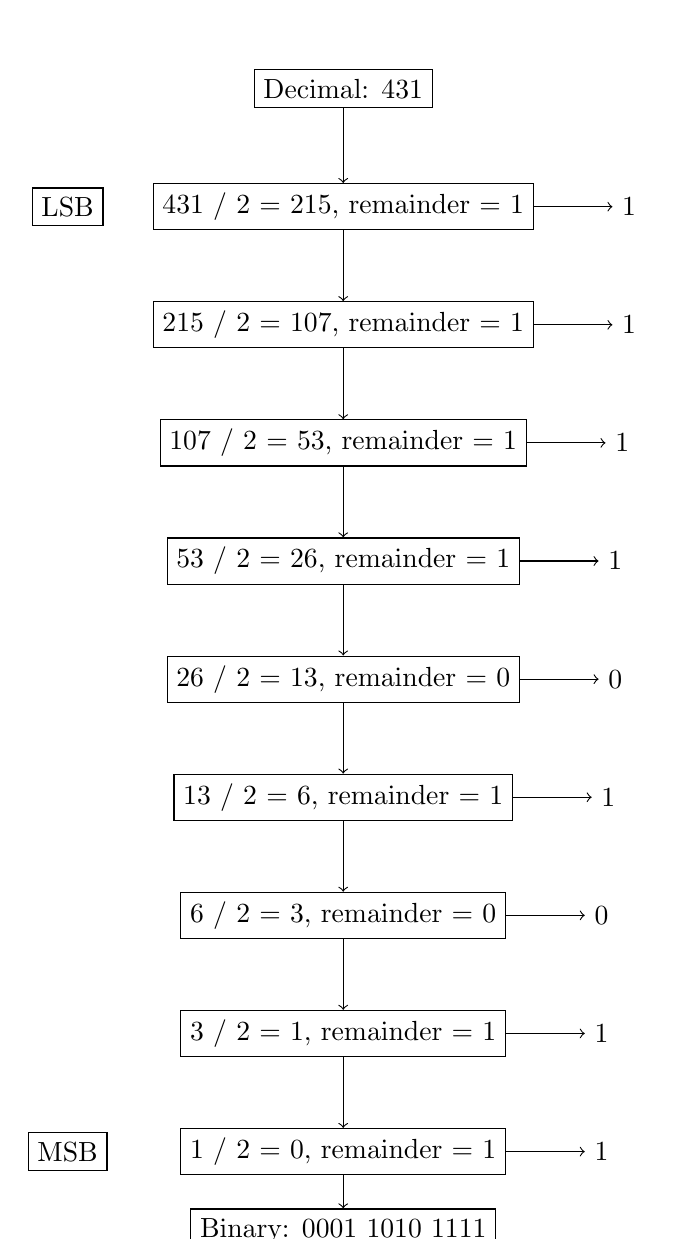
\begin{tikzpicture}[node distance=1.5cm]
                    \node (start) [rectangle, draw] {Decimal: 431};
                    \node (div1) [rectangle, draw, below of=start] {431 / 2 = 215, remainder = 1};
                    \node (div2) [rectangle, draw, below of=div1] {215 / 2 = 107, remainder = 1};
                    \node (div3) [rectangle, draw, below of=div2] {107 / 2 = 53, remainder = 1};
                    \node (div4) [rectangle, draw, below of=div3] {53 / 2 = 26, remainder = 1};
                    \node (div5) [rectangle, draw, below of=div4] {26 / 2 = 13, remainder = 0};
                    \node (div6) [rectangle, draw, below of=div5] {13 / 2 = 6, remainder = 1};
                    \node (div7) [rectangle, draw, below of=div6] {6 / 2 = 3, remainder = 0};
                    \node (div8) [rectangle, draw, below of=div7] {3 / 2 = 1, remainder = 1};
                    \node (div9) [rectangle, draw, below of=div8] {1 / 2 = 0, remainder = 1};

                    \node(lsb) [rectangle, draw, left of=div1, xshift=-2cm] {LSB};
                    \node(msb) [rectangle, draw, left of=div9, xshift=-2cm] {MSB};

                    \node (binary) [rectangle, draw, below of=div8, yshift=-1cm] {Binary: 0001 1010 1111};

                    \draw[->] (start) -- (div1);
                    \draw[->] (div1) -- (div2);
                    \draw[->] (div2) -- (div3);
                    \draw[->] (div3) -- (div4);
                    \draw[->] (div4) -- (div5);
                    \draw[->] (div5) -- (div6);
                    \draw[->] (div6) -- (div7);
                    \draw[->] (div7) -- (div8);
                    \draw[->] (div8) -- (div9);
                    \draw[->] (div9) -- (binary);


                    \draw[->] (div1.east) -- ++(1cm,0) node[right] {1};
                    \draw[->] (div2.east) -- ++(1cm,0) node[right] {1};
                    \draw[->] (div3.east) -- ++(1cm,0) node[right] {1};
                    \draw[->] (div4.east) -- ++(1cm,0) node[right] {1};
                    \draw[->] (div5.east) -- ++(1cm,0) node[right] {0};
                    \draw[->] (div6.east) -- ++(1cm,0) node[right] {1};
                    \draw[->] (div7.east) -- ++(1cm,0) node[right] {0};
                    \draw[->] (div8.east) -- ++(1cm,0) node[right] {1};
                    \draw[->] (div9.east) -- ++(1cm,0) node[right] {1};

                \end{tikzpicture}
                
            \end{center}
            \vspace{1cm}
            The binary representation of \(431_{10}\) is \(0001 \  1010 \ 1111_2\)
        
    
        \newpage

        \item To hexadecimal \newline
        
        The binary representation of the number was calculated in the previous question as \(0001 \  1010 \ 1111_2\) to convert it to hexadecimal, the binary number is divided into groups that contains 4 digits starting from the LSB.
        \begin{align*}
            0001 \parallel 1010 \parallel 1111 \\
        \end{align*}

        The hexadecimal representations of binary numbers are calculated below: \newline

        \begin{align*}
            0001_2 &= 1_{16} \\
            1010_2 &= A_{16} \\
            1111_2 &= F_{16}
        \end{align*}

        So, the hexadecimal representation is : \newline

        \begin{align*}
            431_{10} = 0001 \ 1010 \ 1111_2 &= 1AF_{16}
        \end{align*}

        

        \item To octal \newline
        
        The binary representation of the number was calculated previously to convert the binary number to octal the digits are grouped into 3 digit groups starting from the LSB.

        \begin{align*}
            000 \parallel 110 \parallel 101 \parallel 111  
        \end{align*}
    
        The octal counterparts of the binary numbers are calculated below: \newline

        \begin{align*}
            000_2 &= 0_8 \\
            110_2 &= 6_8 \\
            101_2 &= 5_8 \\
            111_2 &= 7_8
        \end{align*}

        The leading zeros are omitted. So, the octal representation is calculated as: \newline

        \begin{align*}
            431_{10} = 0001 \ 1010 \ 1111_2 &= 657_8
        \end{align*}
    \end{enumerate}
    \newpage
    

    \item \textbf{Express the following numbers in decimal:} \\
    
    \begin{enumerate}
        \item \((10110.0101)_2\)
        \item \((16.5)_{16}\)
        \item \((26.24)_8\)
        \item \((\text{DADA.B})_{16}\)
        \item \((1010.1101)_2\)
    \end{enumerate}

    \textbf{Solutions:} \newline

    \begin{enumerate}[label=\textbf{\alph*.}]
        \item \((10110.0101)_2\) to decimal \newline
        \begin{align*}
            (10110.0101)_2 &= (1 \times 2^4) + (0 \times 2^3) + (1 \times 2^2) + (1 \times 2^1) + (0 \times 2^0) + (0 \times 2^{-1}) + (1 \times 2^{-2}) + (0 \times 2^{-3}) + (1 \times 2^{-4}) \\
           &= 16 + 0 + 4 + 2 + 0 + 0 + 0.25 + 0 + 0.0625 \\
           &= 22.3125
        \end{align*}

        \item \((16.5)_{16}\) to decimal \newline
        
        \begin{align*}
            (16.5)_{16} &= (1 \times 16^1) + (6 \times 16^0) + \left(5 \times 16^{-1}\right) \\
            &= 16 + 6 + \frac{5}{16} \\
            &= 16 + 6 + 0.3125 \\
            &= 22.3125
        \end{align*}
        

        \item \((26.24)_8\) to decimal \newline
        
        \begin{align*}
            \left(26.24\right)_{8} &= \left(2 \times 8^1\right) + \left(6 \times 8^0\right) + \left(2 \times 8^{-1}\right)+ \left(4 \times 8^{-2}\right) \\
            &= 16 + 6 + 0.25 + 0.0625 \\
            &= 22.3125
        \end{align*}
        
        \item \((\text{DADA.B})_{16}\) to decimal \newline
        
        To convert the hexadecimal number to decimal first the values of hexadecimal letters must be converted to decimal. \newline

        \begin{align*}
            \text{A}_{16} &= 10_{10} \\
            \text{B}_{16} &= 11_{10} \\
            \text{D}_{16} &= 13_{10}
        \end{align*}
        
        \begin{align*}
            \text{DADA.B}_{16} &= (13 \times 16^3) + (10 \times 16^2) + (13 \times 16^1) + (10 \times 16^0) + (11 \times 16^{-1}) \\
            &= (13 \times 4096) + (10 \times 256) + (13 \times 16) + (10 \times 1) + (11 \times 0.0625) \\
            &= 53248 + 2560 + 208 + 10 + 0.6875 \\
            &=56026.6875
        \end{align*}

        \newpage
        \item \((1010.1101)_2\) to decimal \newline
        
        \begin{align*}
            (1010.1101)_2 &= (1 \times 2^3) + (0 \times 2^2) + (1 \times 2^1) + (0 \times 2^0) + (1 \times 2^{-1}) + (1 \times 2^{-2}) + (0 \times 2^{-3}) + (1 \times 2^{-4}) \\
            &= 8 + 0 + 2 + 0 + 0.5 + 0.25+ 0 + 0.0625 \\
            &= 10.8125
        \end{align*}

    \end{enumerate}

    \item \textbf{Convert the following binary numbers to hexadecimal and to decimal:} \newline
    
    \begin{enumerate}[label=\textbf{\alph*.}]
        \item 1.10010
        \item 110.010. Explain why the decimal answer in (b) is 4 times that in (a).
    \end{enumerate}

    \textbf{Solutions:} \newline

    \begin{enumerate}[label=\textbf{\alph*.}]
        \item 1.10010 to hexadecimal and decimal \newline
        \begin{enumerate}[label=\textbf{\roman*.}]
            \item To hexadecimal \newline
            
            To convert the binary number to hexadecimal the number is grouped into 4 digit groups starting from the decimal point. \newline
            \begin{align*}
                0001 \parallel . \parallel 1001 \parallel 0000
            \end{align*}

            The hexadecimal representations are calculated as follows: \newline

            \begin{align*}
                0001_2 &= 1_{16} \\
                1001_2 &= 9_{16} \\
                0000_2 &= 0_{16}
            \end{align*}
            
            So the resukting hexadecimal number is: \newline
        
            \begin{align*}
                (1.10010)_2 = (1.9)_{16}
            \end{align*}

            \item To decimal \newline
            
            \begin{align*}
                (1.10010)_2 &= (1 \times 2^0) + (1 \times 2^{-1}) + (0 \times 2^{-2}) + (0 \times 2^{-3}) + (1 \times 2^{-4}) + (0 \times 2^{-5}) \\
                &= 1 + 0.5 + 0 + 0 + 0.0625 + 0 \\
                &= 1.5625   
            \end{align*}

        \end{enumerate}

        \item 110.010 to hexadecimal and decimal \newline
        
        \begin{enumerate}[label=\textbf{\roman*.}]
            \item To hexadecimal \newline
            
            To convert the binary number to hexadecimal the number is grouped into 4 digit groups starting from the decimal point. \newline

            \begin{align*}
                0110 \parallel . \parallel 0100
            \end{align*}

            The hexadecimal representations are calculated as follows: \newline

            \begin{align*}
                0110_2 &= 6_{16} \\
                0100_2 &= 4_{16}
            \end{align*}

            So the resukting hexadecimal number is: \newline

            \begin{align*}
                (110.010)_2 = (6.4)_{16}
            \end{align*}

            \item To decimal \newline
            
            \begin{align*}
                (110.010)_2 &= (1 \times 2^2) + (1 \times 2^1) + (0 \times 2^0) + (0 \times 2^{-1}) + (1 \times 2^{-2}) + (0 \times 2^{-3}) \\
                &= 4 + 2 + 0 + 0 + 0.25 + 0 \\
                &= 6.25
            \end{align*}
        
            The decimal answer in (b) is 4 times  that in (a) because the binary number in (b) is left shifted by 2 bits with moving the decimal point right by 2 bits. If the decimal point is moved right by n bits the resultant number is multiplied by \(2^n\). If we consider a decimal number \(AB.CD_2\) the decimal equivalent is calculated as: \newline

            \begin{align*}
                \text{AB.CD}_2 = (A \times 2^1) + (B \times 2^0) + (C \times 2^{-1}) + (D \times 2^{-2})
            \end{align*}

            If we left shift the number by 2 bits the number becomes \(\text{ABCD}\) and the decimal equivalent is calculated as: \newline

            \begin{align*}
                \text{ABCD}_2 = (A \times 2^3) + (B \times 2^2) + (C \times 2^1) + (D \times 2^0)
            \end{align*}

            By factoring out the resultant equation by \(2^2\) we get: \newline

            \begin{align*}
                \text{ABCD}_2 = 2^2 \times \left((A \times 2^1) + (B \times 2^0) + (C \times 2^{-1}) + (D \times 2^{-2})\right)
            \end{align*}

            So, the decimal equivalent of the left shifted number is 4 times the decimal equivalent of the original number. Also it can be seen from the powers of 2 is increased by 2 in the left shifted number.

        \end{enumerate}

   

    \end{enumerate}

    \newpage

    \item \textbf{Draw truth table of the Boolean function \(f(x,y,z) = x'y + z\)} \newline
    
    \textbf{Solution:} \newline

    \renewcommand{\arraystretch}{2} % Adjust the value as needed

    \begin{table}[h]
        \centering
        \captionsetup{belowskip=10pt} % Add space below caption
        \caption{Truth Table for the Function \(f(x,y,z) = x'y + z\)} 
        
        \label{tab:my-table}
        \begin{tabular}{cccc} % Adjust column specifier for better spacing
            \toprule
            \multicolumn{1}{c}{\(x\)} & 
            \multicolumn{1}{c}{\(y\)} & 
            \multicolumn{1}{c}{\(z\)} & 
            \multicolumn{1}{c}{\(f(x,y,z)\)} \\ 
            \midrule
            0 & 0 & 0 & 0 \\ \hline
            0 & 0 & 1 & 1 \\ \hline
            0 & 1 & 0 & 1 \\ \hline
            0 & 1 & 1 & 1 \\ \hline
            1 & 0 & 0 & 0 \\ \hline
            1 & 0 & 1 & 1 \\ \hline
            1 & 1 & 0 & 0 \\ \hline
            1 & 1 & 1 & 1 \\ \hline
            \bottomrule
        \end{tabular}
    \end{table}




\end{enumerate}

\newpage

\section*{Part 2}

As per instructions, Xilinx ISE 14.7 webpack was installed using the Windows 10 version, the program runs on Oracle Virtual Box using Oracle Linux to mitigate compatibility issues. I have previously attempted to install the software to my computer runnnig Fedora 40 but the signal simulator tool Xilinx ISim was not running properly. 

\subsection*{Importing Files}

From Ninova "\verb|AND_gate.v|" and "\verb|AND_gate_tb.vhd|" files were downloaded and imported into the project navigator using add source command. 
By further inspection the file "\verb|AND_gate.v|" was found to be a Verilog file and the file "\verb|AND_gate_tb.vhd|" was found to be a VHDL file for testing the Verilog file.

\subsubsection*{AND\_gate.v}

The Verilog file "\verb|AND_gate.v|" contains the following code:

\begin{center} % Center the entire code block
    \lstset{
  caption= AND\_gate.v, 
  basicstyle=\footnotesize, frame=tb,
  xleftmargin=.2\textwidth, xrightmargin=.2\textwidth
}
    \lstinputlisting[style=verilogstyle]{../AND_gate.v}

    \end{center}

The verilog file describes an AND gate with two inputs and one output. The module is named as \verb|AND_gate| in the first line starting the module via the module keyword. The inputs are declared in line 2 as \verb|a| and \verb|b| and the output is declared in line 3 as \verb|c|. In the line 5 the assign statement is used for assigning the output \verb|c| to the result of and operation between the inputs. The final argument \verb|endmodule| is used for declaring the end of the module.


\subsubsection*{AND\_gate\_tb.vhd}

The VHDL file "\verb|AND_gate_tb.vhd|" contains the following code:

\begin{center} % Center the entire code block
    \lstset{
  caption= AND\_gate\_tb.vhd, 
  basicstyle=\footnotesize, frame=tb,
  xleftmargin=.2\textwidth, xrightmargin=.2\textwidth
}
    \lstinputlisting[style=vhdlstyle]{../AND_gate_tb.vhd}

\end{center}

This file is a testbench described in VHDL which is used for testing and verifying the functionality of the Verilog file. 

In the first line the IEEE library was imported and in the second line \verb|STD_LOGIC_1164| package was made available. The \verb|STD_LOGIC_1164| package contains the IEEE standard 1164 which includes the definitions of logic values used for signals. \\

In the 4th and 5th lines an ENTITY named \verb|AND_gate_tb| is declared without any ports. \\

In the 7th line the ARCHITECTURE of the ENTITY is declared as \verb|behavioral|. \\

Between the lines 11 and 17 the \verb|AND_gate| component is declared with the ports \verb|IN1|, \verb|IN2| and \verb|OUT1|.\\
The lines 21 and 22 initialize the to the value of \verb|0|.

Between the lines 30 and 34 the unit under test is is instantiated with the name \verb|uut| and the ports are connected to the signals \verb|IN1| and \verb|IN2| and the output is connected to the signal \verb|OUT1|.\\

Process and begin statements are used for beginning a process block. A process block in VHDL is a sequential block that executes when the signals change.

The process simply begins by waiting 10 nanoseconds.

The following lines assign \verb|IN1| and \verb|IN2| 1 and 0 respectively. 

After waiting for 10 nanoseconds again the values of \verb|IN1| and \verb|IN2| are changed to 0 and 1 respectively.

After another 10 nanoseconds the values of \verb|IN1| and \verb|IN2| are changed to 1 and 1 respectively.

Finally waiting after 10 nanoseconds the values of \verb|IN1| and \verb|IN2| are changed to 0 and 0 respectively. 

The wait at the and of the process waits indefinitely.

\subsection*{The Error In Code}

The error in code is that in the testbench the signals were defined as \verb|IN1|, \verb|IN2| and \verb|OUT1| but in the Verilog module \verb|AND_gate| the signals were defined as \verb|a|, \verb|b| and \verb|c|. The signals in the testbench must be defined as the same as the signals in the module.
PORT MAP in the VHDL testbench or the Verilog module input, output names can be changed to correct the issues. I have changed the Verilog code to use \verb|IN1| and \verb|IN2| instead of \verb|a| and \verb|b| and \verb|OUT1| instead of \verb|c|.

The corrected code can be seen below:

\begin{center} % Center the entire code block
    \lstset{
  caption= Corrected AND\_gate.v, 
  basicstyle=\footnotesize, frame=tb,
  xleftmargin=.2\textwidth, xrightmargin=.2\textwidth
}
    \lstinputlisting[style=verilogstyle]{../AND_gate_corrected.v}

\end{center}




\subsection*{Viewing the RTL Schematic}

RTL is an abbreviation for Register Transfer Level. An RTL schematic graphically represents the digital circuit.

Using the Xilinx ISE the RTL schematic of the Verilog module \verb|AND_gate| was viewed. The RTL schematics with different settings are shown below.


\begin{figure}[H] % Forces the figure to stay here
    \centering
    \includegraphics[width=0.5\textwidth]{rtlall.png} % Change to your image name
    \caption{RTL Schematic of the Verilog Module AND\_gate. Every option is selected from the visualisation menu.} % Improved caption
    \label{fig:rtlall} % Label for referencing
\end{figure}

\begin{figure}[H] % Forces the figure to stay here
    \centering
    \includegraphics[width=0.3\textwidth]{ANDGATEPRIMITIVE1.png} % Adjusted width for consistency
    \caption{RTL Schematic of the Verilog Module AND\_gate with only the option "AND\_gate primitive" selected.} % Improved caption
    \label{fig:and_gate_primitive} % Added label for referencing
\end{figure}

\begin{figure}[H] % Forces the figure to stay here
    \centering
    \includegraphics[width=0.5\textwidth]{ANDGATEWITHSIGNALS.png} % Consistent width
    \caption{RTL Schematic of the Verilog Module AND\_gate with "AND\_gate with all signals" selected.} % Improved caption
    \label{fig:and_gate_with_signals} % Added label for referencing
\end{figure}

\subsection*{Simulating the Design}

The file \verb|AND_gate_tb.vhd| was selected and "Simulate Behavioral Model" was run the results generated are shown below.

\begin{figure}[H]
    \centering
    \includegraphics[width=\textwidth]{simt_0.png}
    \caption{Simulation Results of the Testbench of the AND\_gate Module at t=0.}
    \label{fig:simulation0}
\end{figure}

In the VHDL testbench code the initialization of the signals \verb|IN1| and \verb|IN2| were set to 0. The expected output for an AND gate is 0 when both inputs are 0. The simulation between 0-10ns verifies this.



\begin{figure}[H]
    \centering
    \includegraphics[width=\textwidth]{simat15ns.png}
    \caption{Simulation Results of the Testbench of the AND\_gate Module at t=15ns.}
    \label{fig:simulation15}
\end{figure}

In the VHDL testbench the code sets the signals \verb|IN1| and \verb|IN2| to 1 and 0 respectively. The expected output for an AND gate is 0 when one of the inputs is 0. The simulation between 10-20ns verifies this.

\begin{figure}[H]
    \centering
    \includegraphics[width=\textwidth]{simat25ns.png}
    \caption{Simulation Results of the Testbench of the AND\_gate Module at t=25ns.}
    \label{fig:sim25}

\end{figure}

In the VHDL testbench the code sets the signals \verb|IN1| and \verb|IN2| to 0 and 1 respectively. The expected output for an AND gate is 0 when one of the inputs is 0. The simulation between 20-30ns verifies this.



\begin{figure}[H]
    \centering
    \includegraphics[width=\textwidth]{simat35ns.png}
    \caption{Simulation Results of the Testbench of the AND\_gate Module at t=35ns.}
    \label{fig:sim35}

\end{figure}

In the VHDL testbench the code sets the signals \verb|IN1| and \verb|IN2| to 1. The expected output for an AND gate is 1 when two of the inputs are 1. The simulation between 30-40ns verifies this.


\subsection*{Results}

The simulation successfully verifies and tests the AND gate module described in the Verilog code the behavior of the AND gate is consistent with the expected behavior. The RTL schematics were viewed at different levels and included in the report also the simulation graph is included between 0-60ns.



\end{document}